


\documentclass[]{article}
\usepackage{graphicx}
\usepackage{amsmath}
\usepackage{amssymb}
\usepackage{amsfonts}
\usepackage{fancyhdr}
\usepackage[headheight=65pt,tmargin=150pt,headsep=95pt]{geometry}
\usepackage{ragged2e}
\usepackage{array}
\usepackage{tabularx}



\graphicspath{{./images/}}

\pagestyle{myheadings}
\markright {2663452m\hfill 22/01/23\hfill}

\title{\vspace{-8em}
\textbf{Weakly Interacting Massive Particles (WIMPs) 
and the Higgs Boson as Dark Matter Candidates }}
\author{2663452m (University of Glasgow)}
\date{30/01/2023}


\begin{document}

\maketitle
Since the first half of the 20th century the phenomena of Dark Matter (DM) has eluded \
some of the greatest minds in physics. The existence of DM was first 
proposed by Fritz Zwicky in 1933, due to observations of galaxy clusters that suggest
an undetected mass, DM.$^1$ This conclusion was inferred as the velocity the visible matter was
moving at should have exceeded the escape velocity of the cluster. 
This was later confirmed in the 1970s by Astronomer Vera Rubin, who found that
the rotation curves of spiral galaxies had a flat profile,$^1$ which indicated 
that there was more mass present in the outer reaches of the galaxies than 
was visible. From these observations the search for DM began, and today 
there are many theories as to what DM is.
\parskip 0.2cm


One of the difficulties in the search for DM is that the particles are thought 
to be Weakly Interacting Massive Particles (WIMP's)$^2$ as well as being non-relativistic.
Due to this difficulty in the direct observation of WIMP's, researchers
at the Large Hadron Collider (LHC) at CERN, have been using the ATLAS and CMS 
detectors to indirectly observe WIMP's by observing the loss of energy during the 
collision of two protons, as there is some amount of missing transverse energy ($E^{miss}_{T} $)
after the collision (see Figure 1)$^2$, and due to the law of the conservation of energy
this must be accounted for, and is thought to be DM in the form of WIMP's. 



\begin{figure}[h]
\centering  
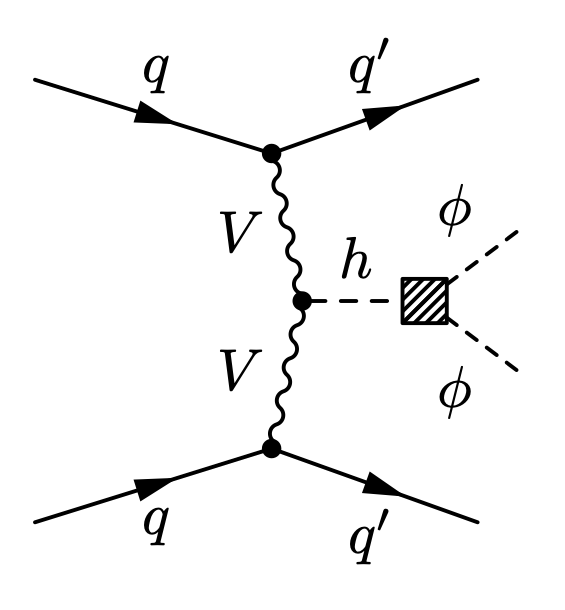
\includegraphics[width=0.3\textwidth]{images/Feynman Diagrams of missing Tranverse energy.png}
\caption{Higgs production (h) due to Vector Boson Fusion with a pair of top quarks ((q) on the left) resulting in Vector Bosons (V) colliding and forming a Higgs Boson and Missing transverse energy $E^{miss}_{T} (\phi)$ in the ATLAS detector.$^3$}
\label{fig:missing_energy}
\end{figure}

\par
However, one of the more successful direct detection of DM comes from the 
XENON1T$^4$ experiment in which liquid Xenon (LXe) is used to detect WIMP's.
This experiment uses the measured electron recoil caused by these particles
to determine their mass. 
\par
\parskip 0.2cm

\parskip 0.2cm
From these detections of particles that may be DM, Theoretical Physicists have
been constructing models to help explain this data, such as the Minimal Supersymmetric
Standard Model (MSSM),$^5$ which is a model that extends the Standard Model (SM) by
adding new particles, such as the Higgs Boson, and the Higgsino, (which is a
lighter version of the Higgs Boson) and these particles including those in the SM 
thought to have a symmetric particle associated with them.$^3$ The Higgs Boson is thought to be the particle
that gives mass to the other particles in the SM, and is a potential 
candidate for DM. During observations of the Higgs Boson there has been increasing
evidence that the Higgs Boson may be a DM candidate
as it has a relatively high mass in the GeV range, and has been observed
to be electrically neutral with a spin state of 0.$^3$
\parskip 0.2cm
\newpage
\noindent 
\subsection*{[4] E. Aprile et al. (2018) Dark Matter Search Results from a One Ton-Year Exposure of XENON1T}

\parskip 0.2cm
In this article the XENON collaboration present the results of their data analysis
of the XENON1T experiment carried out at the Gran Sasso National Laboratory in Italy.
The experiment uses  1 tonne of liquid Xenon (LXe) to detect WIMP's, and the 
electron recoil caused by these particles is measured by the detector. This was an 
important experiment in the search for DM as it introduces tighter tolerances on what 
a DM candidate should be, and provided experimental evidence that the Higgs Boson
may be a DM candidate.\parskip 0.2cm

\noindent 
\subsection*{[2] Daniel S. Levin (2016) Search for Dark Matter in ATLAS In LHC Run-2}
\parskip 0.2cm
This second source discusses the search of DM through collisions carried out at the Large 
Hadron Collider (LHC) at CERN, making use of the ATLAS and CMS detectors 
(A Toroidal LHC Apparatus and Compact Muon Solenoid respectively).
From these collisions (typically of high energy protons) the ATLAS and CMS detectors
observed a loss of energy in the form of missing transverse energy ($E^{miss}_{T} $)
giving rise to a potential DM candidate, as the energy was escaping without 
detections suggesting that they are particles with no electromagnetic influence 
and are therefore DM. These escaping particles are thought to be the Higgs Boson 
as it has a relatively high mass and would result in a substantial loss of energy
in a given system. However, it is unclear if the Higgs Boson is as 
described in the typical standard model, as it is possible to be a result of a more 
complicated model of the subatomic world, such as the Minimal Supersymmetric Standard Model (MSSM)
or a model which implies the existence of more dimensions. With how recent this paper 
is it provides a new set of data from the LHC run 2 that can be used to further refine 
what a DM candidate may be, as we further await LHC run 3 later this decade with 
significant improvements that are planned along with new, more sensitive detectors\parskip 0.2cm 

\noindent 

 
\subsection*{[5] Vasiliki A Mitsou (2013) Overview of searches for dark matter at the LHC}
\parskip 0.2cm
Similar to the source above, this article analyses the data collected by the
ATLAS and CMS detectors at the LHC, and how the observations of collisions results in
missing transverse energy. However, it considers that this missing energy may be
a more general group of particles, classified as Weakly Interacting Massive Particles (WIMP's).
This group also included the Higgs Boson, and provides a rough outline for what 
the mass of these particles may be by considering the results obtained 
from the XENON1T experiment. This article provides a powerful insight into how these
two separate attempts at detecting DM are related and can be used together 
to provide a more accurate picture of what DM may be.



\section*{References}

[1] W. J. G. de Blok et al. High-Resolution Rotation Curves of Low Surface Brightness
Galaxies. II. Mass Models AJ 122 2396 (2001) DOI 10.1086/323450

\par
\noindent
[2] Levin, Daniel. Search for Dark Matter in ATLAS In LHC Run-2
ATL-PHYS-PROC-2016-100 (2016) https://cds.cern.ch/record/2206864




\par
\noindent
[3] Argyropoulos, S.; Brandt, O.; Haisch, U. Collider Searches for Dark Matter 
through the Higgs Lens. Symmetry 13, 2406. (2021)
https://doi.org/10.3390/sym13122406 \par
\noindent
[4] Aprile, E. et al. Dark Matter Search Results from a One Ton-Year Exposure of XENON1T
Phys. Rev. Lett. 121 11 (2018) https://link.aps.org/doi/10.1103/PhysRevLett.121.111302


\par
\noindent
[5] Vasiliki A Mitsou. Overview of searches for dark matter at the LHC. J. Phys.: Conf. Ser. 651 012023 (2015) 
DOI 10.1088/1742-6596/651/1/012023

\par
\noindent
[6] Bertone, G., Tait, T.M.P. A new era in the search for dark matter. 
Nature 562, 51–56 (2018). https://doi.org/10.1038/s41586-018-0542-z
\par
\noindent
[7] ATLAS and CMS release results of most comprehensive studies ye of higgs boson's
properties (2022)
https://home.cern/news/news/physics/atlas-and-cms-release-results-most-comprehensive-studies-yet-higgs-bosons
\par
\noindent
[8] El-Kosseifi, R., Kneur, JL., Moultaka, G. et al. The Higgs boson mass as 
fundamental parameter of the minimal supersymmetric standard model. Eur. Phys. 
J. C 82, 657 (2022). https://doi.org/10.1140/epjc/s10052-022-10606-4 



\end{document}